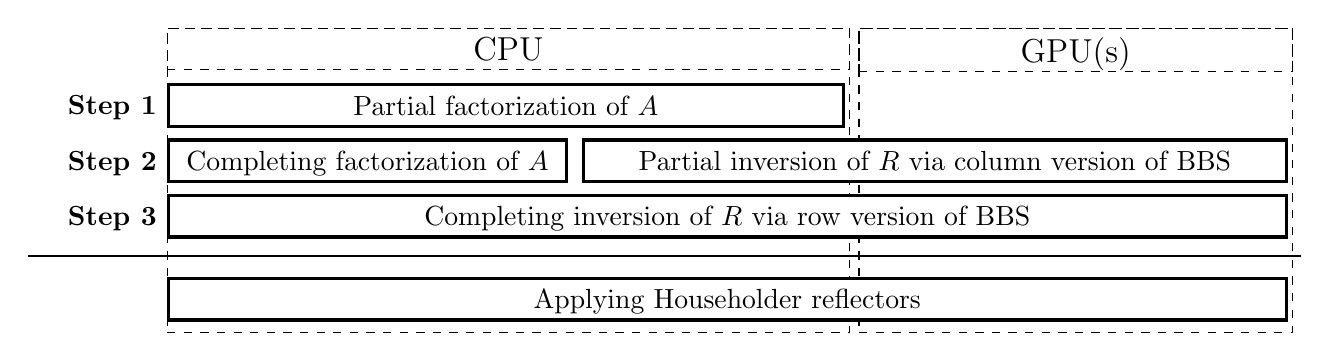
\begin{tikzpicture}[>=latex,text depth=0.0ex]

  \tikzstyle{algBlockStyle}  = [rectangle,fill=white,very thick,inner sep=2pt,minimum height=1.5em,draw,anchor=north west,text centered,]

  \node[text width=24em,minimum height=11em,anchor=north west,dashed,draw] at (0,2em) {};
  \node[text width=24em,anchor=north west,text centered,dashed,draw] at (0,2em) {\large CPU};
  \node[text width=15em,minimum height=11em,anchor=north west,dashed,draw] at (25em,2em) {};
  \node[text width=15em,anchor=north west,text centered,dashed,draw] at (25em,2em) {\large GPU(s)};
  % . 
  \node[algBlockStyle,text width=24em] (BSOFTRI1) {%
    Partial factorization of $A$
    % (without updating the last block column)
  };
  \node [anchor=east] at (BSOFTRI1.west) {{\bf Step 1}};

  \node[algBlockStyle,text width=14em] (BSOFTRI2) at (0,-2em) {%
    Completing factorization of $A$
  };
  \node[algBlockStyle,text width=25em] at (15em,-2em) {
    Partial inversion of $R$ via column version of BBS
  };
  \node [anchor=east] at (BSOFTRI2.west) {{\bf Step 2}};

  \node[algBlockStyle,text width=40em] (BSOFTRI3) at (0em,-4em) {
    Completing inversion of $R$ via row version of BBS
  };
  \node [anchor=east] at (BSOFTRI3.west) {{\bf Step 3}};
  
  \node[algBlockStyle,text width=40em] (BSOI) at (0em,-7em) {
    Applying Householder reflectors
  };

  \draw (-5em,-6.25em) -- (41em,-6.25em);
  \path (BSOFTRI2.west) +(-4em,0) node [anchor=south,rotate=90] {\large \Bsoftri};
  \path (BSOI.west) +(-4em,0) node [anchor=south,rotate=90] {\large \Bsoi};

\end{tikzpicture}
